\documentclass[11pt]{article}
\usepackage{pillplan}
% Generated by pillplan_tools.catalog.build. Do not edit by hand.
\newcommand{\CatalogDrugs}{43}
\newcommand{\CatalogIngredients}{43}
\newcommand{\CatalogIngredientsWithLimit}{35}
\newcommand{\CatalogClasses}{34}
\newcommand{\CatalogAreas}{8}
\newcommand{\CatalogTimingRules}{9}
\newcommand{\CatalogWarnings}{9}
\newcommand{\CatalogAreaPie}{
  13/Heart and circulation,
  6/Pain and inflammation,
  5/Infection,
  4/Allergy and breathing,
  4/Diabetes,
  4/Mental health and sleep,
  4/Other,
  3/Stomach
}

% Generated by scripts/collect-metrics.mjs. Do not edit by hand.
\newcommand{\MetricInitialJsGzip}{92.8}
\newcommand{\MetricInitialJsBrotli}{80.7}
\newcommand{\MetricCssGzip}{7.3}
\newcommand{\MetricFonts}{43.9}
\newcommand{\MetricLazyGzip}{21.4}
\newcommand{\MetricWebTests}{114}
\newcommand{\MetricWebTestFiles}{11}
\newcommand{\MetricPyTests}{15}
\newcommand{\MetricAllTests}{129}

\IfFileExists{generated/lighthouse.tex}{% Generated by scripts/lighthouse-to-tex.py. Do not edit by hand.
\newcommand{\LighthousePerformance}{100}
\newcommand{\LighthouseAccessibility}{100}
\newcommand{\LighthouseBestPractices}{100}
\newcommand{\LighthouseSeo}{100}
\newcommand{\LighthouseLcp}{0.8 s}
\newcommand{\LighthouseTbt}{0 ms}
\newcommand{\LighthouseCls}{0}
\newcommand{\LighthouseNote}{local production build, mobile, LCP 0.8 s, blocking time 0 ms, layout shift 0}
}{
  \newcommand{\LighthousePerformance}{0}\newcommand{\LighthouseAccessibility}{0}
  \newcommand{\LighthouseBestPractices}{0}\newcommand{\LighthouseSeo}{0}
  \newcommand{\LighthouseNote}{not measured yet}}

\begin{document}

\thispagestyle{empty}
\begin{tikzpicture}[remember picture, overlay]
  \fill[amber] ([xshift=22mm,yshift=-22mm]current page.north west) rectangle ++(14mm,-2.2mm);
\end{tikzpicture}
\vspace*{8mm}
{\fontsize{34}{38}\selectfont\bfseries PillPlan}\par
\vspace{2mm}
{\Large Technical Documentation}\par
\vspace{4mm}
{\color{inkmuted}Architecture, design system, data, testing, performance and deployment.}\par
\vspace{6mm}
\begin{tabular}{@{}ll@{}}
\textbf{Version} & 2.0, 2 November 2026 \\
\textbf{Stack} & React 19, TypeScript 6, Vite 8, Python 3.12 with Pydantic 2 \\
\textbf{Hosting} & Netlify, static files only \\
\textbf{Repository} & \url{https://github.com/4arkeinlvy/pillplan} \\
\end{tabular}
\vspace{6mm}

\begin{note}
\textbf{At a glance.} \CatalogDrugs\ medicines, \MetricAllTests\ automated tests, \MetricInitialJsGzip\ KB of initial JavaScript, no server and no database. Everything the user types stays in their own browser.
\end{note}

\tableofcontents
\newpage

\section{System context}
PillPlan is a static website. Python runs only on the developer machine and in CI, where it checks the drug data and writes the JSON file the app loads. In the browser, the React app does all the work.

\begin{center}
\begin{tikzpicture}[node distance=9mm and 14mm]
  \node[datafile] (csv) {data-src/*.csv\\\footnotesize edited in Excel};
  \node[box, right=of csv] (py) {Python tools\\\footnotesize Pydantic checks};
  \node[datafile, right=of py] (json) {catalog.json};
  \node[accent, below=14mm of json] (app) {React app\\\footnotesize in the browser};
  \node[box, left=of app] (netlify) {Netlify CDN\\\footnotesize static files};
  \node[box, left=of netlify] (git) {GitHub\\\footnotesize code and CI};
  \node[box, below=12mm of app] (user) {Pharmacist\\or student};
  \node[box, right=12mm of app] (ls) {localStorage\\\footnotesize this device only};
  \node[box, left=12mm of user] (paper) {Printed chart\\or PDF};
  \node[box, left=12mm of paper] (patient) {Patient};

  \draw[flow] (csv) -- (py);
  \draw[flow] (py) -- node[lbl, above] {writes} (json);
  \draw[flow] (json) -- node[lbl, right] {bundled} (app);
  \draw[flow] (git) -- node[lbl, above] {build} (netlify);
  \draw[flow] (netlify) -- node[lbl, above] {serves} (app);
  \draw[flow, <->] (app) -- (ls);
  \draw[flow, <->] (user) -- (app);
  \draw[flow] (user) -- (paper);
  \draw[flow] (paper) -- (patient);
\end{tikzpicture}
\end{center}

\section{Architecture: a modular monolith}
The app is \textbf{one codebase, one build and one deploy}, split into five feature modules with strict borders. Each module has a public \texttt{index.ts}. Other code may import only from that file. A shared kernel holds what every module agrees on.

\begin{center}
\begin{tikzpicture}[node distance=10mm and 6mm]
  \node[accent, minimum width=60mm] (app) {app shell \footnotesize(layout, startup)};
  \node[feature, below=16mm of app, xshift=-48mm] (catalog) {catalog\\\footnotesize search, data};
  \node[feature, right=of catalog] (medicines) {medicines\\\footnotesize plan, form, list};
  \node[feature, right=of medicines] (schedule) {schedule\\\footnotesize chart, tracker};
  \node[feature, below=12mm of medicines, xshift=-17mm] (safety) {safety\\\footnotesize checks, notes};
  \node[feature, right=of safety] (storage) {storage\\\footnotesize save, export};
  \node[soft, below=12mm of safety, xshift=17mm, minimum width=110mm] (shared) {shared kernel: time slots, dose format, strings, icons, UI primitives, tokens};

  \begin{scope}[on background layer]
    \node[draw=rule, dashed, rounded corners=2pt, inner sep=5mm, fit=(catalog) (schedule) (safety) (storage), label={[font=\footnotesize, text=inkmuted]north east:features}] {};
  \end{scope}

  \draw[dep] (app) -- (catalog);
  \draw[dep] (app) -- (medicines);
  \draw[dep] (app) -- (schedule);
  \draw[dep] (app.south west) to[bend right=25] (safety.west);
  \draw[dep] (app.south east) to[bend left=25] (storage.east);
  \draw[flow] (medicines) -- (catalog);
  \draw[flow] (schedule) -- (medicines);
  \draw[flow] (safety) -- (medicines);
  \draw[flow] (safety) -- (catalog);
  \draw[flow] (storage) -- (medicines);
\end{tikzpicture}
\end{center}
Black arrows are allowed dependencies between features. They always point one way, so there are no cycles.

\subsection{Rules the linter enforces}
\begin{tabularx}{\linewidth}{@{}>{\bfseries}p{48mm}X@{}}
\toprule
Rule & ESLint check \\
\midrule
Use a feature through its door & \texttt{@/features/x/inner/file} is refused. Only \texttt{@/features/x} is allowed. \\
No reaching across with paths & \texttt{../../other-feature} is refused inside features. \\
Shared stays generic & \texttt{shared} may not import any feature or the app shell. \\
No cycles & \texttt{import-x/no-cycle}. \\
No raw HTML injection & \texttt{react/no-danger}. \\
\bottomrule
\end{tabularx}

\subsection{Shared kernel: two languages}
\texttt{shared/i18n} holds one dictionary per language, \texttt{en.ts} and \texttt{id.ts}. The Indonesian one is typed as \texttt{Strings}, so TypeScript refuses a missing or misspelled key. Logic functions take the dictionary as a parameter (\texttt{validateMedicine(m, t)}, \texttt{runSafetyChecks(meds, catalog, t, lang)}); components read it with \texttt{useI18n()}. Catalog text such as advice and warnings is stored as \texttt{\{en, id\}} pairs. Numbers follow the locale: \texttt{0.5 mg} and \texttt{4,000 mg} in English, \texttt{0,5 mg} and \texttt{4.000 mg} in Indonesian, always with a leading zero and no trailing zero.

\subsection{Inside a feature}
Every feature uses the same layout:
\begin{itemize}
  \item \texttt{model.ts}: types.
  \item \texttt{logic/}: pure TypeScript functions with no React, each with tests.
  \item \texttt{ui/}: thin React components, each with its own CSS Module file. Class names are scoped to that component and Vite merges all styles into one small CSS file.
  \item \texttt{index.ts}: the public API.
\end{itemize}

\section{Data pipeline}
\begin{center}
\begin{tikzpicture}[node distance=8mm and 9mm]
  \node[datafile] (d) {drugs.csv};
  \node[datafile, below=4mm of d] (i) {ingredients.csv};
  \node[datafile, below=4mm of i] (w) {warnings.csv};
  \node[box, right=12mm of i] (read) {csv\_source\\\footnotesize split lists};
  \node[box, right=of read] (model) {Pydantic models\\\footnotesize types and shapes};
  \node[box, right=of model] (cat) {Catalog check\\\footnotesize cross references};
  \node[datafile, above right=4mm and 10mm of cat] (json) {catalog.json};
  \node[datafile, below right=4mm and 10mm of cat] (tex) {catalog-stats.tex};
  \node[box, below=16mm of model, fill=highlight] (ci) {CI: build {-}{-}check fails if out of date};

  \draw[flow] (d.east) -- (read);
  \draw[flow] (i) -- (read);
  \draw[flow] (w.east) -- (read);
  \draw[flow] (read) -- (model);
  \draw[flow] (model) -- (cat);
  \draw[flow] (cat) |- (json);
  \draw[flow] (cat) |- (tex);
  \draw[dep, dashed] (ci) -| (cat);
\end{tikzpicture}
\end{center}

The catalog check refuses:
\begin{itemize}
  \item a duplicate id, an unknown ingredient or an unknown warning;
  \item a strength that does not give one amount per ingredient;
  \item a unit that does not match its ingredient;
  \item a single tablet stronger than the usual daily maximum;
  \item any em or en dash in the text.
\end{itemize}

\subsection{What is in the catalog}
\begin{center}
\begin{tikzpicture}
  \CatalogAreaPie{text=legend, radius=2.6, sum=auto, after number={},
       color={ink, amber, stickerblue, inkmuted, stickeryellow, alert, rule, desk}}
\end{tikzpicture}
\end{center}
\CatalogDrugs\ medicines in \CatalogClasses\ drug classes and \CatalogAreas\ areas. \CatalogIngredientsWithLimit\ of \CatalogIngredients\ ingredients have a usual daily maximum, \CatalogTimingRules\ medicines have a best time of day, and there are \CatalogWarnings\ warning stickers.

\section{Signa entry}
\texttt{parseSigna()} in \texttt{features/medicines/logic/signa.ts} is a pure function with 34 tests. It reads Latin and Indonesian aturan pakai and returns times, amount, form, food, ``when needed'' and a list of words it did not understand, which the form shows as ``Check: \dots''.

\begin{tabularx}{\linewidth}{@{}>{\ttfamily}p{44mm}X@{}}
\toprule
\textrm{\textbf{Signa}} & \textbf{Meaning in PillPlan} \\
\midrule
1 dd, 1x, o.d., q.d. & once a day: the drug's usual time, or Pagi \\
2 dd, 2x, b.i.d., tiap 12 jam & Pagi and Malam \\
3 dd, 3x, t.i.d., tiap 8 jam, q8h & Pagi, Siang and Malam \\
4 dd, 4x, q.i.d., tiap 6 jam & Pagi, Siang, Malam and Sebelum tidur \\
o.m., pagi & Pagi (omni mane) \\
o.n., malam & Malam (omni nocte) \\
h.s., sebelum tidur & Sebelum tidur (hora somni) \\
a.c., sebelum makan & before food (ante coenam) \\
p.c., d.c., sesudah/saat makan & with or after food (post or durante coenam) \\
p.r.n., s.o.s., bila perlu, k/p & when needed; ``3 dd 1 prn'' means at most 3 a day \\
1, \textonehalf, 1/2, 0,5, I, II, s & amount; s (semis) is \textonehalf \\
tab, caps, cth, C, gtt & tablet, capsule, 5 mL, 15 mL, drops \\
\bottomrule
\end{tabularx}

More than 4 doses a day (for example \texttt{tiap 4 jam}) is never guessed: the parser flags it for the apoteker.

\section{Data model}
\begin{center}
\begin{tikzpicture}[
  cls/.style={draw=ink, line width=0.9pt, rectangle split, rectangle split parts=2,
    rectangle split part fill={ink, white}, font=\footnotesize, align=left, inner sep=4pt,
    text width=40mm},
  node distance=10mm and 12mm]
  \node[cls] (drug) {\textcolor{white}{\textbf{Drug}}\nodepart{second}id, name, brands\\ingredients[], strengths[][]\\drugClass, area, form, unit\\defaultTimes, bestTimes\\food, warnings[], advice, source};
  \node[cls, right=of drug] (ing) {\textcolor{white}{\textbf{Ingredient}}\nodepart{second}id, name, unit\\usualMaxDaily, source};
  \node[cls, below=of ing] (warn) {\textcolor{white}{\textbf{WarningLabel}}\nodepart{second}id, short, text\\icon, sticker color};
  \node[cls, below=of drug] (med) {\textcolor{white}{\textbf{Medicine}}\nodepart{second}id, drugId or null\\name, strength\\ingredientAmounts[]\\amount, form, times[]\\prn, prnMaxPerDay, food\\warnings[], purpose, advice\\pill: shape, color};
  \node[cls, below=of med] (plan) {\textcolor{white}{\textbf{PlanState}}\nodepart{second}patientName\\medicines[]\\tracker: start, popped[]};
  \node[cls, right=of plan] (note) {\textcolor{white}{\textbf{SafetyNote}}\nodepart{second}id, kind, severity\\medicineIds[], title, detail};

  \draw[flow] (drug) -- node[lbl, above] {1..n} (ing);
  \draw[flow] (drug.east) ++(0,-6mm) -| node[lbl, pos=0.7] {0..n} (warn.north);
  \draw[flow] (med) -- node[lbl, right] {0..1 drugId} (drug);
  \draw[flow] (plan) -- node[lbl, right] {0..n} (med);
  \draw[flow, dashed] (note) -- node[lbl, above] {about} (plan);
\end{tikzpicture}
\end{center}

\section{Adding a medicine}
\begin{center}
\begin{tikzpicture}[x=1mm, y=1mm, font=\footnotesize]
  \foreach \x/\n in {0/User, 30/DrugSearch, 60/MedicineForm, 90/planReducer, 120/ChartSheet and SafetyNotes, 150/usePersistence} {
    \node[box, minimum width=24mm, text width=22mm] (h\x) at (\x,0) {\n};
    \draw[rule, line width=1pt] (\x,-5) -- (\x,-92);
  }
  \newcommand{\msg}[4]{\draw[flow] (#1,#3) -- node[lbl, above] {#4} (#2,#3);}
  \msg{0}{30}{-12}{types ``metf''}
  \msg{30}{60}{-22}{onPick(drug)}
  \node[lbl, anchor=west] at (61,-29) {prefill from catalog};
  \msg{0}{60}{-38}{set times, food}
  \msg{60}{90}{-48}{dispatch add}
  \node[lbl, anchor=west] at (91,-55) {new PlanState};
  \msg{90}{120}{-62}{re-render}
  \node[lbl, anchor=west] at (121,-69) {runSafetyChecks};
  \msg{90}{150}{-78}{effect: save}
  \draw[flow, dashed] (120,-88) -- node[lbl, above] {sees chart} (0,-88);
\end{tikzpicture}
\end{center}
The add is wrapped in a View Transition, so the new row slides in. Browsers without View Transitions simply update.

\section{Saving and loading}
\begin{center}
\begin{tikzpicture}[node distance=10mm and 22mm, every state/.style={draw=ink, line width=0.9pt, minimum size=16mm, font=\footnotesize, align=center}]
  \node[state, initial, initial text={start}] (read) {read\\storage};
  \node[state, right=of read] (parse) {parse and\\validate};
  \node[state, accepting, right=of parse, fill=highlight] (restored) {restored};
  \node[state, below=of read] (blocked) {storage\\blocked};
  \node[state, below=of parse] (fresh) {new chart};
  \node[state, below=of restored] (notice) {new chart\\+ notice};

  \draw[flow] (read) -- node[lbl, above] {found} (parse);
  \draw[flow] (parse) -- node[lbl, above] {valid} (restored);
  \draw[flow] (parse) -- node[lbl, right] {invalid} (notice);
  \draw[flow] (read) -- node[lbl, right] {blocked} (blocked);
  \draw[flow] (read) -- node[lbl, pos=0.5, sloped] {empty} (fresh);
  \draw[flow] (blocked) -- node[lbl, above] {export only} (fresh);
\end{tikzpicture}
\end{center}
The browser copy and an exported file use the same envelope: \texttt{\{app, version, savedAt, plan\}}. Valibot checks it before use. Pill colors must be plain hex values, because they end up in an SVG fill.

\section{Phone reminders}
\texttt{buildIcs()} writes an iCalendar (RFC 5545) file in the browser: one daily event per time of day in use, each with an alarm, repeating for 30 days, in floating local time so it rings at the same clock time wherever the phone is. Text is escaped and long lines are folded at 75 bytes. The default times are 07:00, 12:00, 19:00 and 21:00 and can be changed before download. When-needed medicines get no reminder.

\section{Design system}
\subsection{Direction: a dispensing label}
The look comes from real pharmacy objects, not from a template:
\begin{itemize}
  \item white label paper, black ink and ruled lines;
  \item one amber accent, the color of prescription bottles;
  \item warning stickers in the colors of auxiliary labels;
  \item a blister pack for the tracker.
\end{itemize}

\subsection{Color tokens}
\begin{tabularx}{\linewidth}{@{}l l X l@{}}
\toprule
Token & Hex & Use & Contrast on white \\
\midrule
\textcolor{ink}{\rule{5mm}{3mm}} \texttt{ink} & \texttt{\#141414} & Text and rules & 18.4 : 1 \\
\textcolor{inkmuted}{\rule{5mm}{3mm}} \texttt{ink-muted} & \texttt{\#5A5A5A} & Secondary text & 6.9 : 1 \\
\textcolor{rule}{\rule{5mm}{3mm}} \texttt{rule} & \texttt{\#CFCFCF} & Lines & decorative \\
\textcolor{amber}{\rule{5mm}{3mm}} \texttt{amber} & \texttt{\#B45F06} & Primary buttons, focus ring & 4.6 : 1 \\
\textcolor{alert}{\rule{5mm}{3mm}} \texttt{alert} & \texttt{\#C62828} & Danger, red stickers & 5.6 : 1 \\
\textcolor{stickeryellow}{\rule{5mm}{3mm}} \texttt{sticker-yellow} & \texttt{\#FFD60A} & Caution stickers, black text & 14.0 : 1 (ink) \\
\textcolor{stickerblue}{\rule{5mm}{3mm}} \texttt{sticker-blue} & \texttt{\#1565C0} & Information stickers & 5.8 : 1 \\
\textcolor{highlight}{\rule{5mm}{3mm}} \texttt{highlight} & \texttt{\#FFF1A8} & Spotlight, active option & background \\
\bottomrule
\end{tabularx}

Stickers always combine color, an icon and words:
\sticker{stickeryellow}{ink}{May cause sleepiness} \sticker{alert}{white}{No alcohol} \sticker{stickerblue}{white}{Swallow whole}

\subsection{Typography}
\begin{itemize}
  \item \textbf{Atkinson Hyperlegible Next} for all text. The Braille Institute designed it so letters that are easy to confuse look different.
  \item \texttt{Atkinson Hyperlegible Mono} for dose numbers, where 0, O, 1, l and I must never be confused.
  \item Self-hosted woff2 files, latin only, weights 400 and 700, preloaded.
  \item 18 px base and a 1.25 scale. Print uses 14 pt for names and doses.
\end{itemize}

\subsection{Design rules}
These rules keep the screen calm for a busy counter. Every new screen is checked against them.
\begin{tabularx}{\linewidth}{@{}>{\bfseries}p{40mm}X@{}}
\toprule
Rule & In PillPlan \\
\midrule
One task per area & Left: build the plan. Right: the chart. Everything else (save, PDF, reminders, my drugs) is in the More drawer. Safety notes are one line above the chart until opened. \\
One primary button & Amber only for the main action of a view: Print / PDF, Add to chart, Add to phone calendar. \\
Light controls, strong content & Inputs, chips and buttons have 1 px light grey borders that darken on hover and focus. Strong black lines appear only on the chart sheet. \\
8 px spacing grid & 32 px between sections, 16 px between fields, 6 px from label to control. \\
Type scale & 17 px interface text, 18 px chart text, headings 20, 24 and 32 px. Bold only for names, doses and labels. \\
Touch targets & Every control is at least 44 px tall (WCAG 2.2). \\
Colour budget & About 60\% paper and desk, 30\% ink, at most 10\% amber. A chosen chip is an amber tint, not solid black. \\
Alignment & Fields in a row share one top line. Units sit inside the stepper (``1 tablet'', ``4 kali''), never below it. \\
Motion & 150 to 250 ms, ease out, only when something changes, never looping, off with reduced motion. \\
\bottomrule
\end{tabularx}

\subsection{Icons}
Each time of day has its own shape, so they are never confused: \textbf{Pagi} a sun rising over the horizon, \textbf{Siang} a full sun, \textbf{Malam} a moon with a star, \textbf{Sebelum tidur} a bed with ``z''. When a time chip is switched on, its icon moves once: the sun rays turn, the rising sun lifts, the moon tilts, the ``z'' floats up. The icons are drawn as 24 px SVG with 2 px strokes, so they print sharply.

\subsection{Anti-slop rules}
Taken from Anthropic's \texttt{frontend-design} skill and the \texttt{avoid-ai-design} catalog. PillPlan does not use:
\begin{itemize}
  \item Inter, Roboto or system-ui as the design font;
  \item purple or blue gradients;
  \item the cream, terracotta and serif look;
  \item identical rounded cards with the same soft shadow;
  \item tracked capital labels or one highlighted word in a headline;
  \item fade-up on every section;
  \item sparkle icons or icons in rounded squares;
  \item marketing copy.
\end{itemize}
Motion is used only where it explains a change, built with CSS and the View Transitions API, so it adds no library:

\begin{tabularx}{\linewidth}{@{}>{\bfseries}p{38mm}X@{}}
\toprule
Moment & What moves and why \\
\midrule
Dose stamp & A new dose is pressed into its column like a pharmacy stamp, column by column. It shows where the dose landed. \\
Signa preview & The preview turns bold, a check mark draws itself, and the time chips switch on with their icons moving. \\
Drawer and strip & The More drawer slides in from the right; the safety strip opens downward with a turning chevron. \\
Counseling timeline & A line from sunrise to night; the doses of the current medicine light up and a sun or moon marker slides to the first one. \\
Counseling page turn & Next slides the medicine to the left, Back to the right, so the direction is clear. \\
Note to rows & Pointing at a safety note outlines the medicines it is about and fades the rest. \\
Day ribbon & The bars grow and shrink as medicines are added or removed. \\
Rows and language & Rows slide when added, removed or reordered; the language switch cross-fades. \\
Tracker and notes & A blister bubble pops when ticked; a new safety note arrives like a slapped sticker. \\
\bottomrule
\end{tabularx}

Same-document View Transitions work in Chrome, Edge, Firefox 144+ and Safari 18+; other browsers simply update. All motion is switched off when the device asks for reduced motion.

\subsection{Screens}
\begin{center}
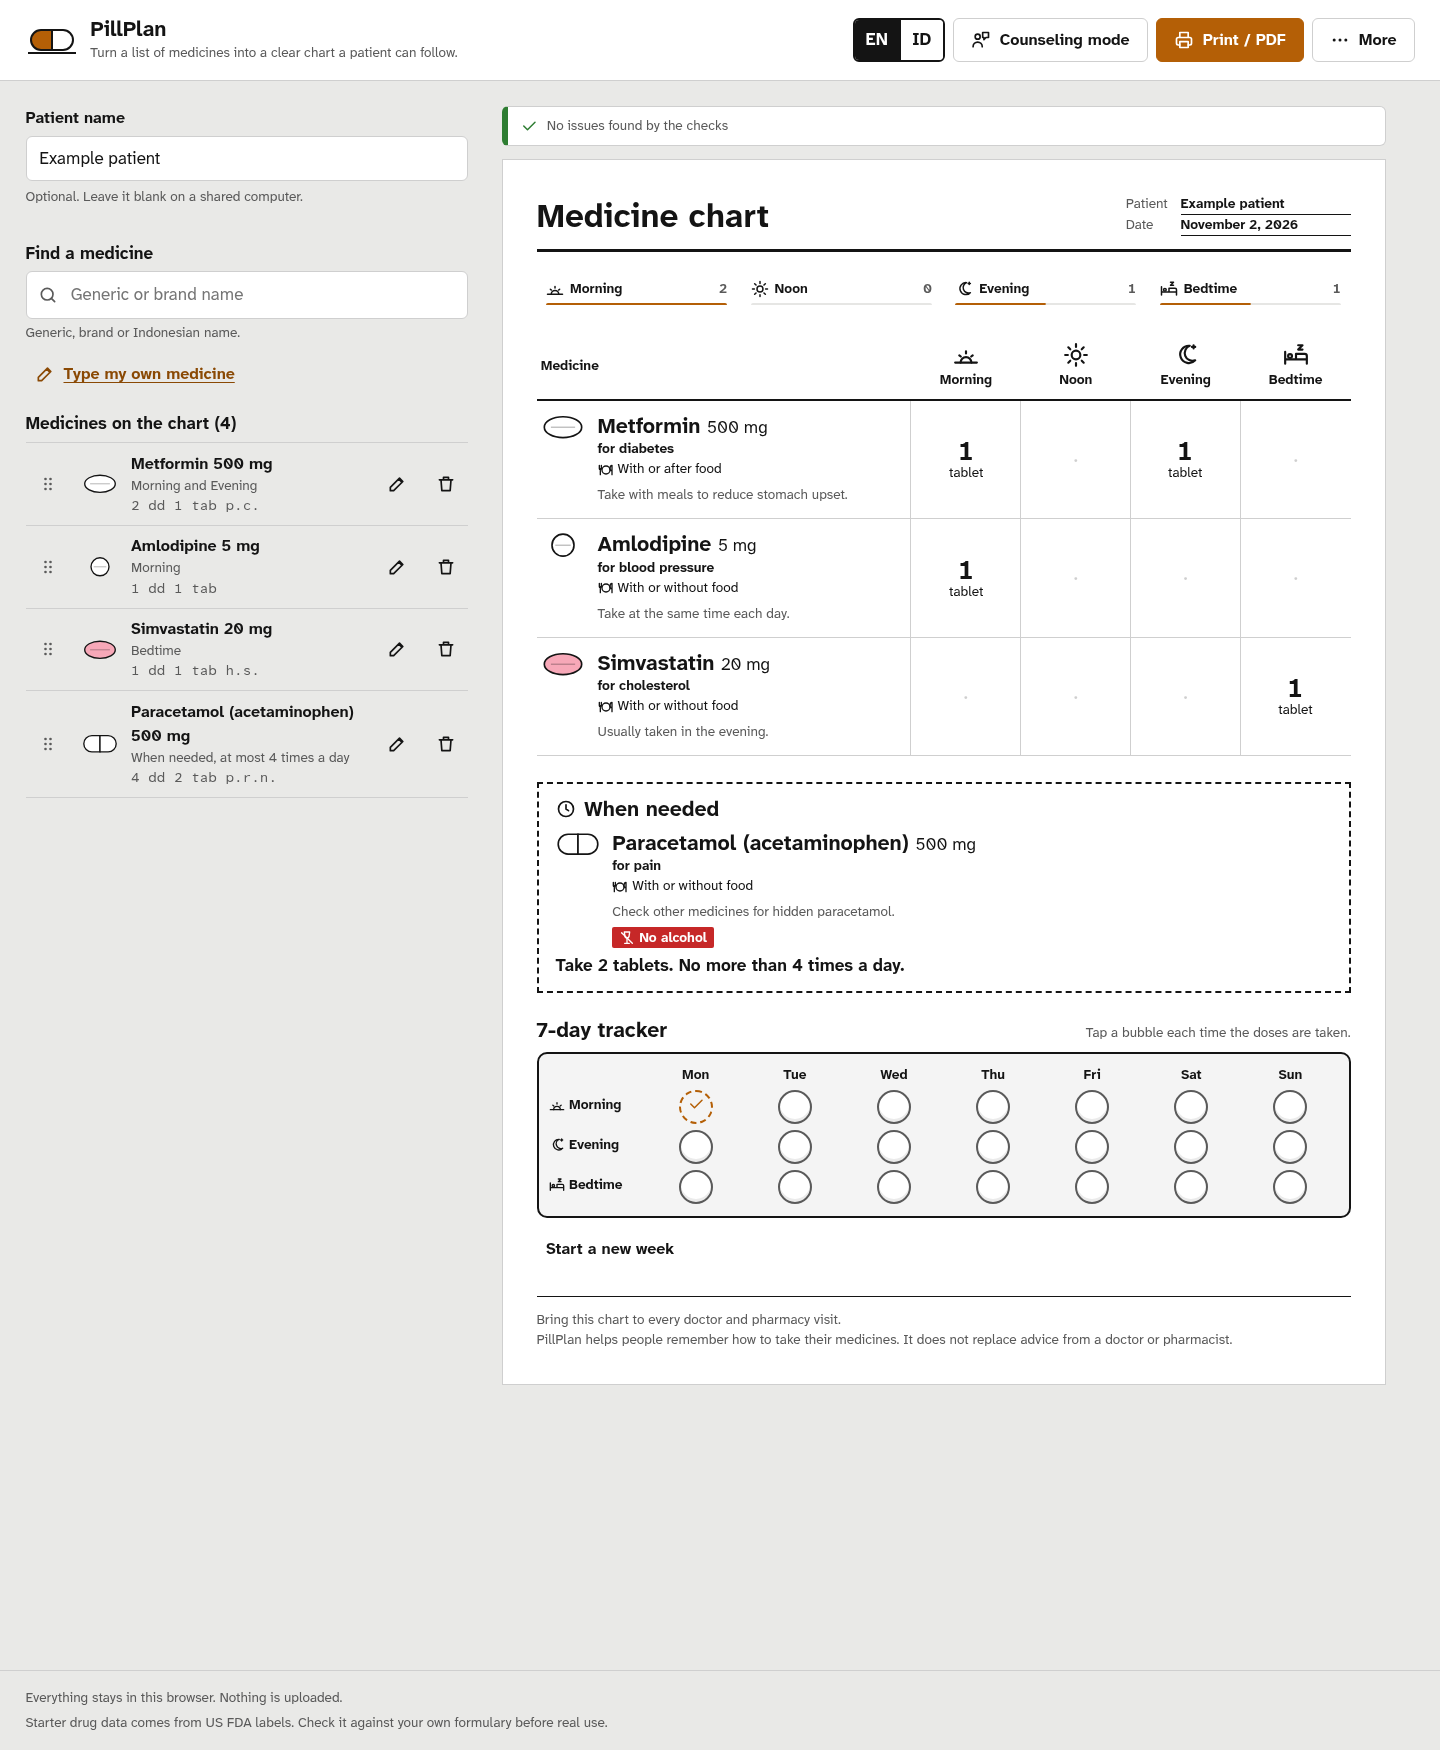
\includegraphics[width=\linewidth]{screenshots/desktop.png}\\[2mm]
{\footnotesize\color{inkmuted}Desktop, 1440 px: form and list on the left, the A4 chart on the right.}
\end{center}
\begin{center}
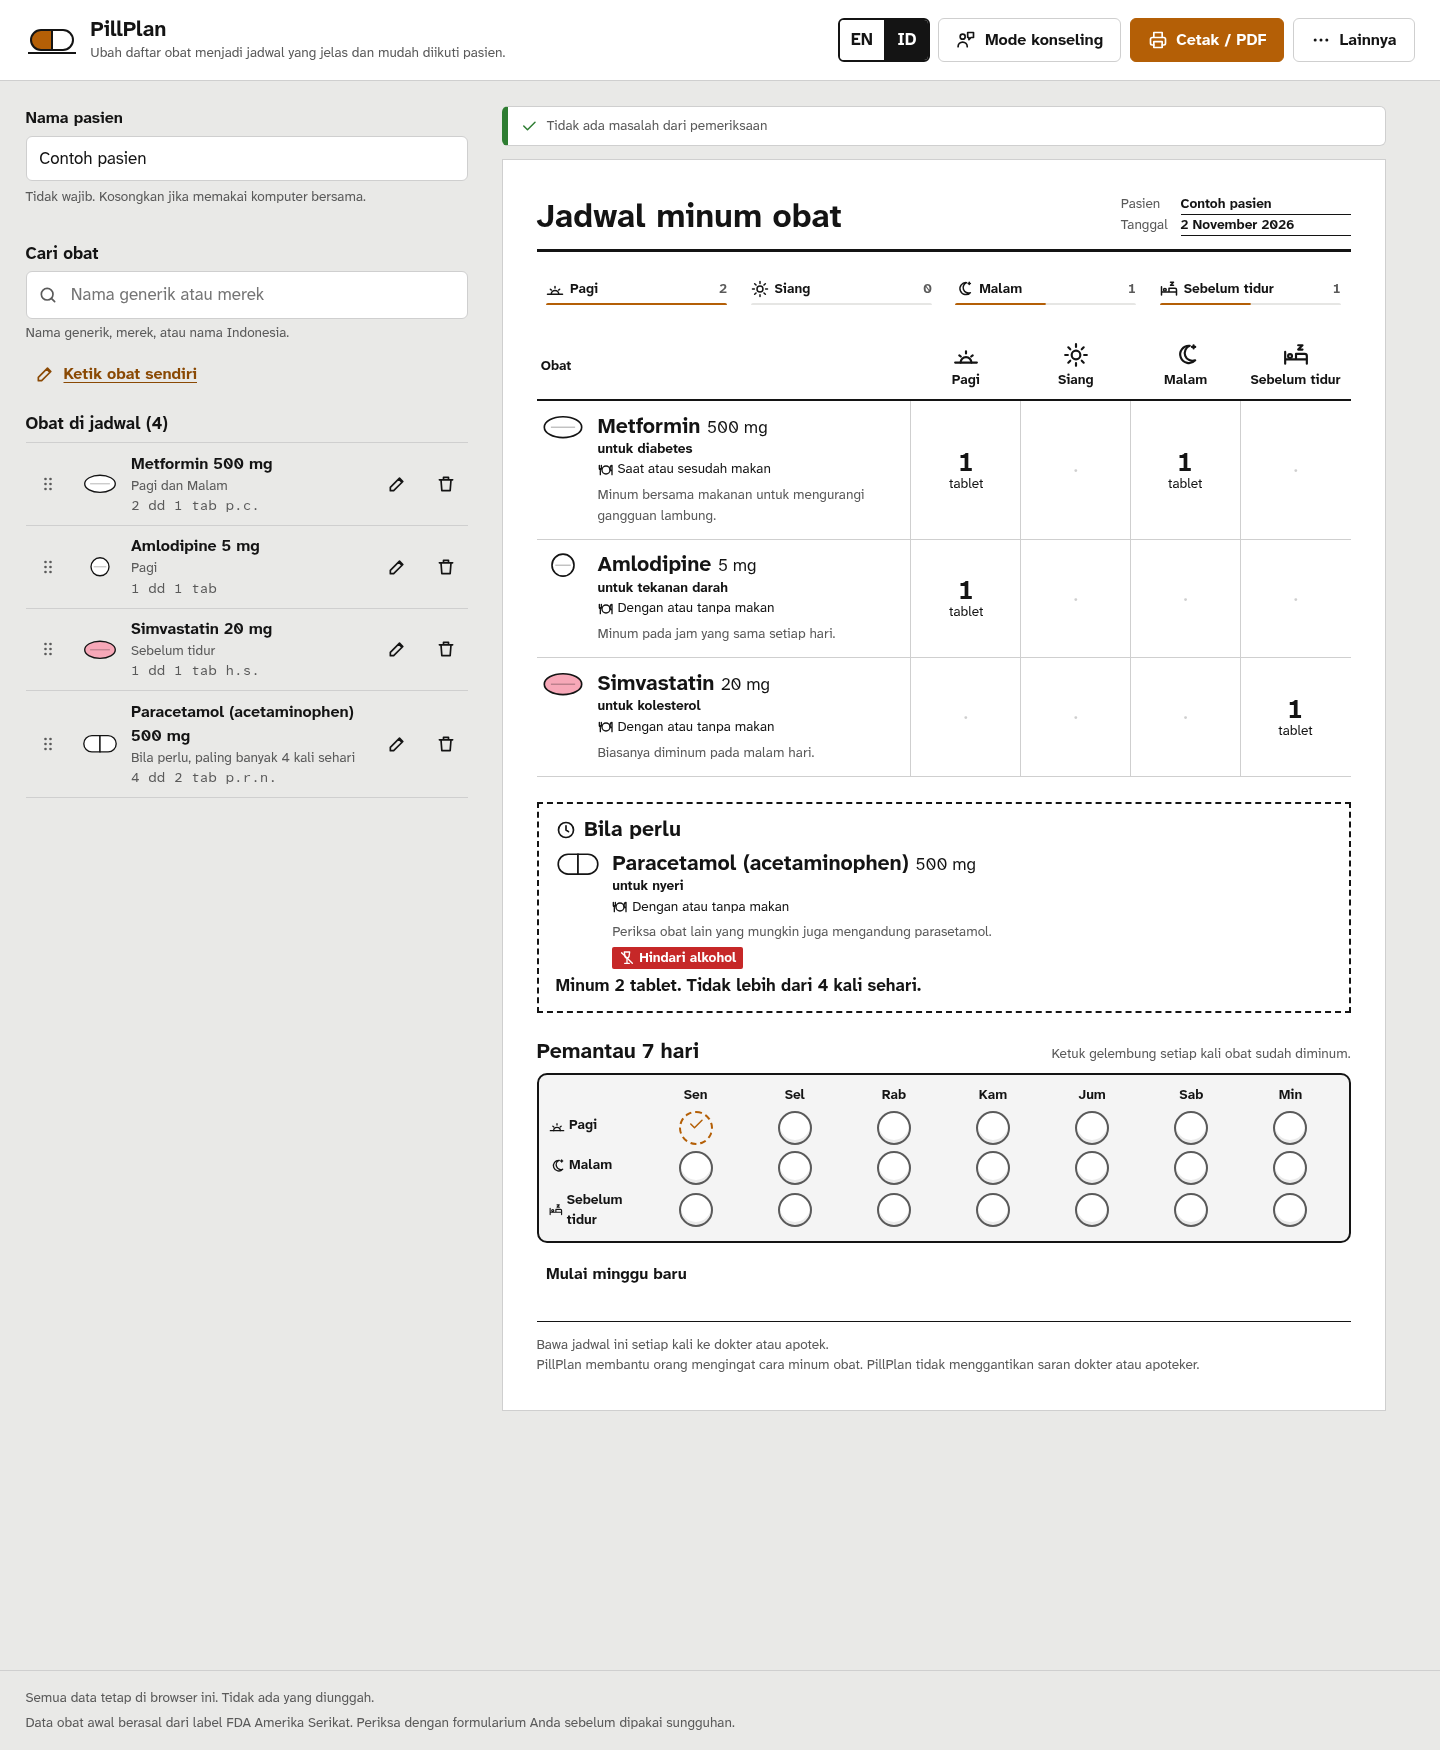
\includegraphics[width=\linewidth]{screenshots/desktop-id.png}\\[2mm]
{\footnotesize\color{inkmuted}The same plan in Indonesian.}
\end{center}
\begin{center}
\begin{minipage}[t]{0.31\linewidth}\centering
  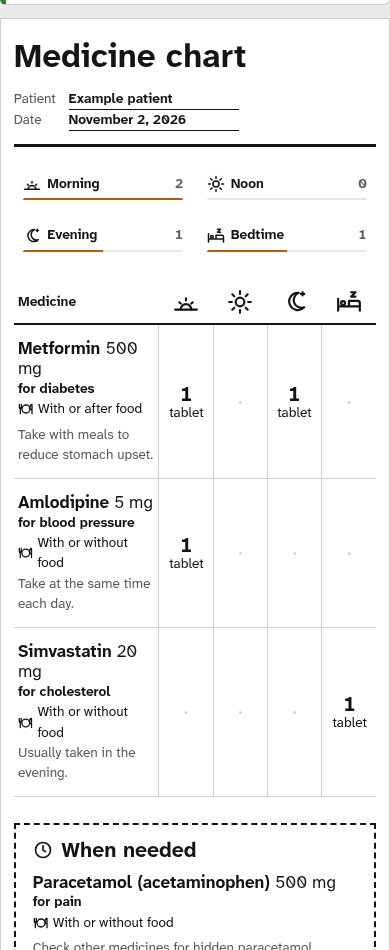
\includegraphics[width=\linewidth]{screenshots/phone-top.png}\\
  {\footnotesize\color{inkmuted}Phone, 390 px}
\end{minipage}\hfill
\begin{minipage}[t]{0.64\linewidth}\centering
  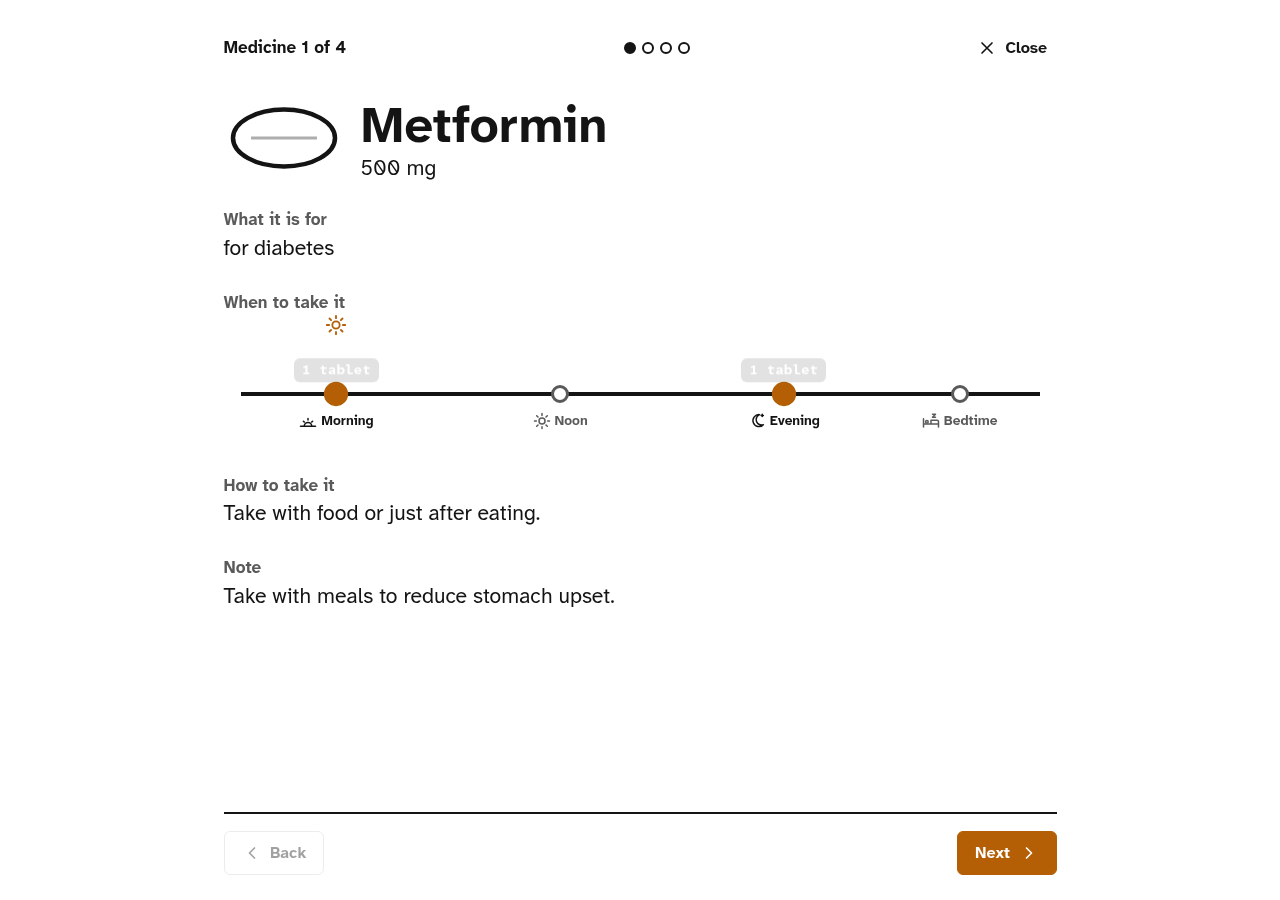
\includegraphics[width=\linewidth]{screenshots/counseling.png}\\
  {\footnotesize\color{inkmuted}Counseling mode}\\[4mm]
  \fbox{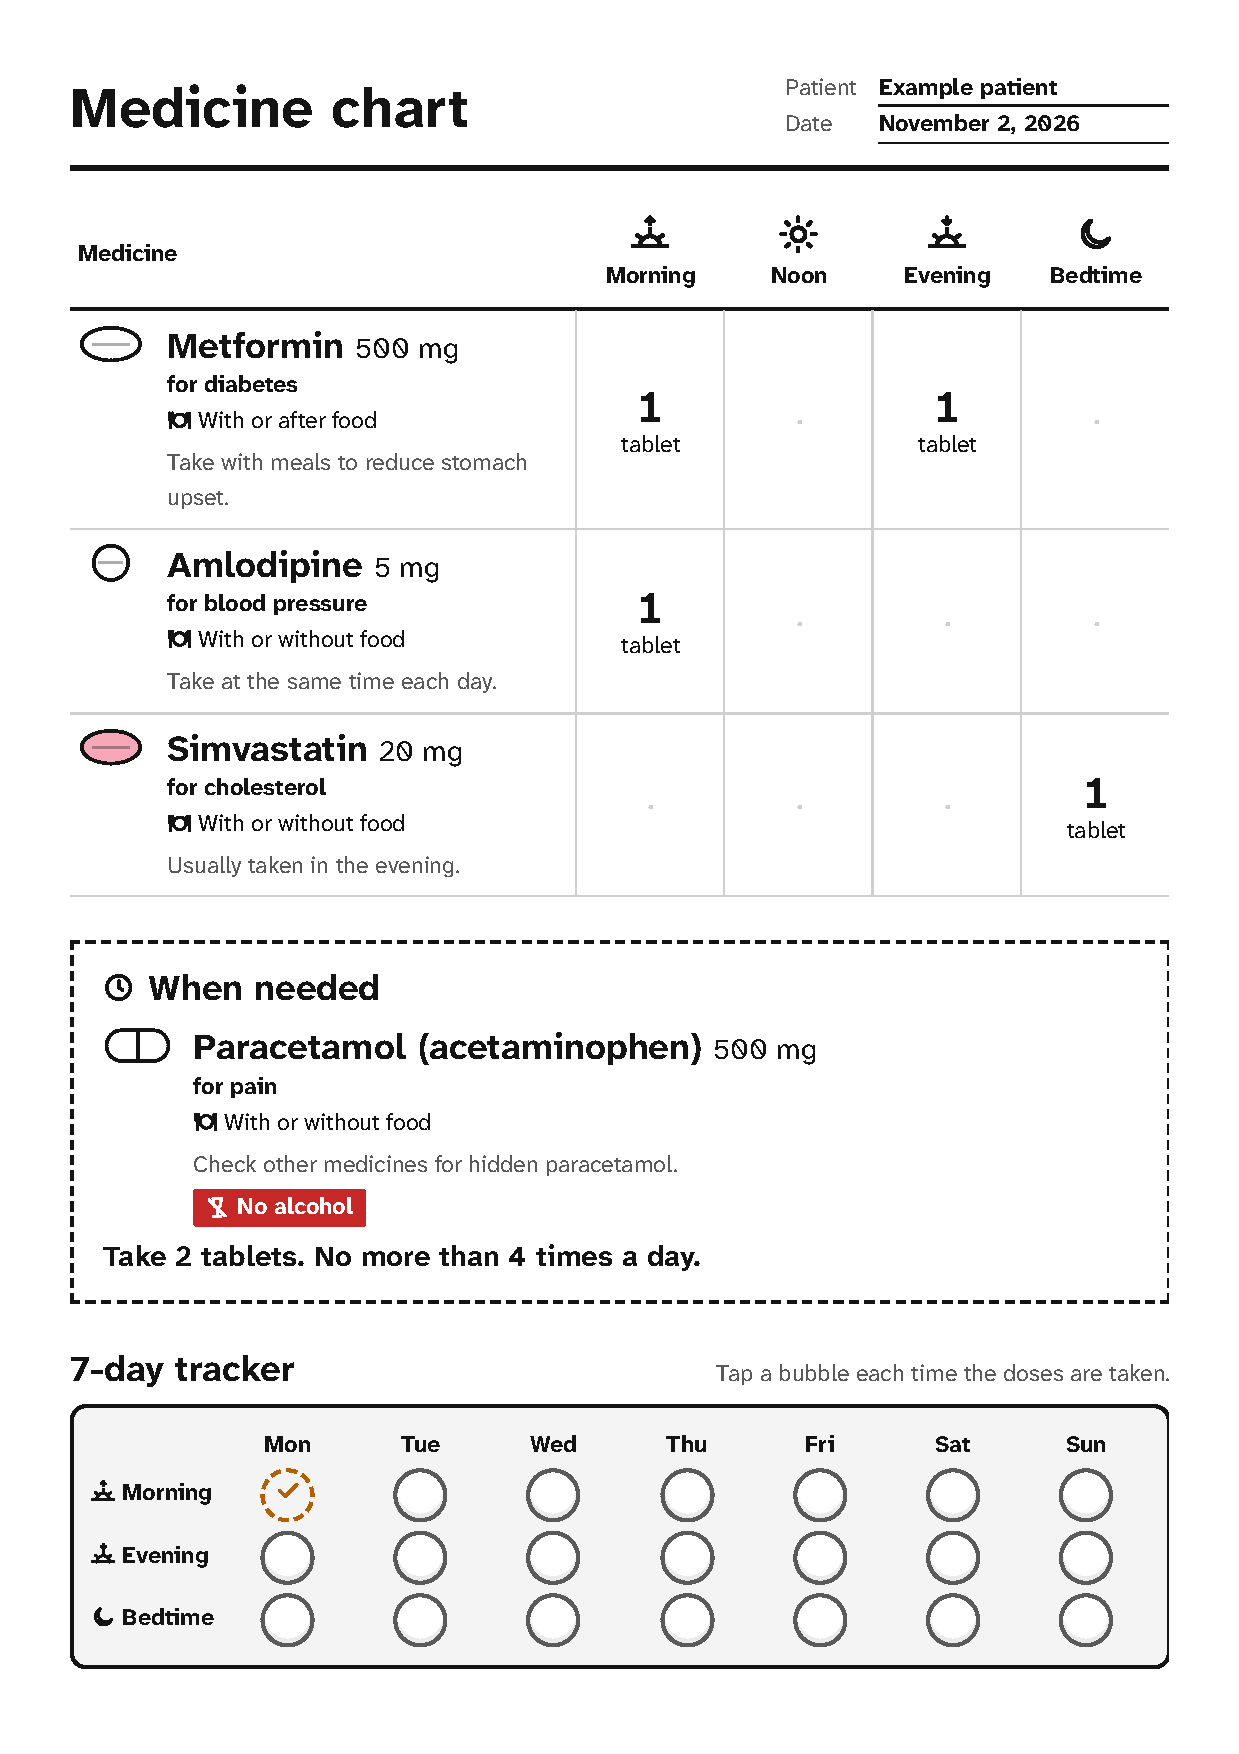
\includegraphics[width=0.62\linewidth,page=1]{screenshots/print.pdf}}\\
  {\footnotesize\color{inkmuted}Print, A4}
\end{minipage}
\end{center}

\section{Safety checks}
\begin{tabularx}{\linewidth}{@{}>{\bfseries}p{38mm} l X@{}}
\toprule
Check & Level & How \\
\midrule
Daily maximum & alert & For each ingredient: amount per unit $\times$ units per dose $\times$ doses per day, summed across every product, compared with the usual maximum. \\
Same ingredient & caution & Two or more products share an ingredient, for example paracetamol in Panadol and Panadol Extra. \\
Same class & caution & Two or more drugs from one specific class, for example two statins. Aspirin and clopidogrel are different classes. \\
Time of day & info & A medicine set outside its best times, for example simvastatin in the morning. \\
Not checked & info & A custom medicine that is not in the catalog. \\
\bottomrule
\end{tabularx}

\section{Testing}
\begin{tabularx}{\linewidth}{@{}>{\bfseries}p{40mm} r X@{}}
\toprule
Suite & Tests & Covers \\
\midrule
Web (Vitest) & \MetricWebTests & Dose formatting, search, reducer, prefill, validation, chart, tracker, safety checks, storage and files, and full user flows in jsdom \\
Data (pytest) & \MetricPyTests & Real catalog validity and every refusal rule \\
\midrule
Total & \MetricAllTests & all passing \\
\bottomrule
\end{tabularx}

The user-flow tests use Testing Library and query by role and accessible name, the same way a screen reader user finds things:
\begin{itemize}
  \item add from search;
  \item hidden paracetamol and undo;
  \item custom medicine;
  \item validation;
  \item counseling mode with arrow keys;
  \item tracker saving;
  \item spotlight;
  \item turning saving off.
\end{itemize}

\section{Performance}
\begin{center}
\begin{tikzpicture}
\begin{axis}[
  xbar, width=0.86\linewidth, height=55mm,
  xlabel={KB}, xmin=0,
  symbolic y coords={Lazy chunks,Fonts,CSS,Initial JS},
  ytick=data, y tick label style={font=\small},
  bar width=4mm, enlarge y limits=0.18,
  legend style={at={(0.98,0.04)}, anchor=south east, font=\footnotesize, draw=none},
  axis line style={ink}, tick style={ink},
  nodes near coords, nodes near coords style={font=\footnotesize},
]
  \addplot[fill=rule, draw=rule] table[x=budget, y=part, col sep=comma] {generated/bundle.csv};
  \addplot[fill=ink, draw=ink] table[x=actual, y=part, col sep=comma] {generated/bundle.csv};
  \legend{Budget, Measured}
\end{axis}
\end{tikzpicture}
\end{center}
JavaScript and CSS sizes are gzip. Initial JavaScript is \MetricInitialJsBrotli\ KB with Brotli, which Netlify serves. The drug list and counseling mode are separate chunks loaded when needed.

\begin{center}
\begin{tikzpicture}
\begin{axis}[
  ybar, width=0.78\linewidth, height=55mm,
  ymin=0, ymax=100, ylabel={Score},
  symbolic x coords={Performance,Accessibility,Best practices,SEO},
  xtick=data, x tick label style={font=\small},
  bar width=12mm, enlarge x limits=0.18,
  nodes near coords, nodes near coords style={font=\small\bfseries},
  axis line style={ink}, tick style={ink},
]
  \addplot[fill=amber, draw=amber] coordinates {
    (Performance,\LighthousePerformance) (Accessibility,\LighthouseAccessibility)
    (Best practices,\LighthouseBestPractices) (SEO,\LighthouseSeo)};
\end{axis}
\end{tikzpicture}\\
{\footnotesize\color{inkmuted}Lighthouse, mobile: \LighthouseNote.}
\end{center}

\section{Security}
\begin{itemize}
  \item No server, database, accounts, cookies, analytics or third-party scripts.
  \item Headers from \texttt{web/public/\_headers} on every response:
\end{itemize}
\begin{tcolorbox}[colback=desk, colframe=desk, arc=0pt, fontupper=\ttfamily\footnotesize]
Content-Security-Policy: default-src 'self'; img-src 'self' data:;\\
\hspace*{4mm}object-src 'none'; base-uri 'none'; frame-ancestors 'none'; form-action 'none'\\
Referrer-Policy: no-referrer\\
X-Content-Type-Options: nosniff\\
Permissions-Policy: camera=(), microphone=(), geolocation=()\\
Cross-Origin-Opener-Policy: same-origin
\end{tcolorbox}
\begin{itemize}
  \item React escapes all text, and \texttt{dangerouslySetInnerHTML} is banned by lint.
  \item Saved data and imported files are validated with Valibot and limited in size.
\end{itemize}

\section{Build, CI and deploy}
\begin{center}
\begin{tikzpicture}[node distance=8mm and 8mm]
  \node[box] (push) {git push};
  \node[box, right=of push] (ci) {GitHub Actions};
  \node[box, above right=2mm and 8mm of ci] (data) {data job\\\footnotesize ruff, pyright, pytest, build {-}{-}check};
  \node[box, right=of ci] (web) {web job\\\footnotesize lint, types, tests, build, size};
  \node[box, below right=2mm and 8mm of ci] (text) {text job\\\footnotesize no dashes};
  \node[accent, right=of web] (net) {Netlify deploy};
  \node[box, right=of net] (cdn) {CDN};
  \draw[flow] (push) -- (ci);
  \draw[flow] (ci) |- (data);
  \draw[flow] (ci) -- (web);
  \draw[flow] (ci) |- (text);
  \draw[flow] (web) -- (net);
  \draw[flow] (net) -- (cdn);
\end{tikzpicture}
\end{center}

\subsection{Deploy step by step}
\begin{enumerate}
  \item \texttt{cd web \&\& npm run build}
  \item \texttt{npx netlify-cli login}, once.
  \item \texttt{npx netlify-cli deploy {-}{-}prod {-}{-}dir web/dist}
  \item Optional: in Netlify, choose \emph{Link repository} so every push deploys. The settings come from \texttt{netlify.toml}.
\end{enumerate}

\section{Editing the drug data}
\begin{enumerate}
  \item Open \texttt{data-src/drugs.csv} in Excel or Google Sheets.
  \item Lists use semicolons, such as \texttt{morning;evening}. Combination strengths use plus, such as \texttt{500+65}. Use \texttt{prn} for when needed.
  \item Every drug needs a \texttt{source}.
  \item Run \texttt{cd tools \&\& uv run python -m pillplan\_tools.catalog.build}. Any mistake is reported with the drug id.
  \item Run the tests, then commit.
\end{enumerate}

\begin{note}[alert]
\textbf{Starter data.} Values are based on US FDA labeling and are for education. Check them against your own formulary before any real use.
\end{note}

\end{document}
